\documentclass[tikz, border=8pt]{standalone}
\usepackage{amsmath}
\usepackage{tikz}
\definecolor{navy}{HTML}{14213D}
\definecolor{teal}{HTML}{0E7C7B}
\definecolor{merah}{HTML}{C0392B}
\definecolor{abu}{HTML}{E8E8E8}

% Rotasi sumbu 45 derajat terhadap titik pusat O.
% Titik P(2,1) pada sumbu biasa, diputar menjadi P' pada sumbu miring.
% Rumus: P'(x cos a - y sin a, x sin a + y cos a), a = 45 derajat.

\definecolor{pagebg}{HTML}{171D2B}
\begin{document}
\pagecolor{pagebg}
\color{white}

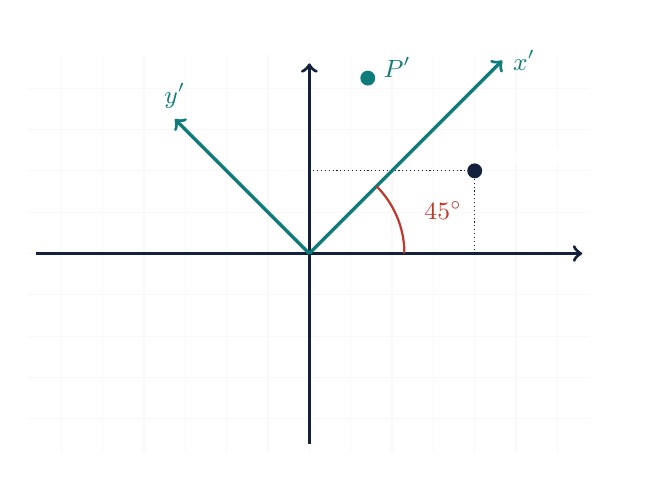
\begin{tikzpicture}[scale=1.05]
  % Grid kecil di sekitar pusat, sumbu asli
  \draw[abu!30, thin] (-3.4,-2.4) grid[step=0.5] (3.4,2.4);
  % Sumbu asli (hitam/navy)
  \draw[navy, very thick, ->] (-3.3,0) -- (3.3,0) node[anchor=west, font=\small\bfseries, white] {$x$};
  \draw[navy, very thick, ->] (0,-2.3) -- (0,2.3) node[anchor=south, font=\small\bfseries, white] {$y$};
  \node[anchor=north east, font=\small\bfseries, white] at (-0.05,-0.05) {$O$};

  % Titik P(2,1) pada sumbu asli
  \fill[navy] (2,1) circle (0.09cm);
  \node[anchor=west, font=\small\bfseries, white] at (2.1,1.15) {$P(2,\,1)$};
  \draw[navy, densely dotted] (2,0) -- (2,1);
  \draw[navy, densely dotted] (0,1) -- (2,1);
  \node[anchor=north, font=\small, white] at (2,-0.12) {$2$};
  \node[anchor=east, font=\small, white] at (-0.12,1) {$1$};

  % Sumbu miring hasil rotasi 45 derajat (teal): cukup sumbu positif
  \draw[teal, very thick, ->, rotate=45] (0,0) -- (3.3,0)
    node[anchor=west, font=\small\bfseries, teal] {$x'$};
  \draw[teal, very thick, ->, rotate=45] (0,0) -- (0,2.3)
    node[anchor=south, font=\small\bfseries, teal] {$y'$};

  % Titik P' hasil rotasi: (2,1) diputar 45 derajat
  % x' = 2cos45 - 1sin45 = (2-1)/sqrt2 ~ 0.707
  % y' = 2sin45 + 1cos45 = (2+1)/sqrt2 ~ 2.121
  \fill[teal] (0.7071,2.1213) circle (0.09cm);
  \node[anchor=west, font=\small\bfseries, teal] at (0.78,2.25) {$P'$};

  % Busur penanda sudut 45 derajat dari sumbu x ke sumbu x'
  \draw[merah, thick] (1.15,0) arc[start angle=0, end angle=45, radius=1.15];
  \node[font=\small\bfseries, merah] at (1.62,0.52) {$45^\circ$};
\end{tikzpicture}

\end{document}
